\documentclass{article}
\usepackage{graphicx} % Required for inserting images
\usepackage{amsmath}   
\usepackage{hyperref}
\usepackage{listings}
\usepackage{rotating}
\usepackage{xcolor}
\usepackage{float}
\usepackage{pdfpages}
\usepackage[a4paper, margin=0.5in]{geometry} 

\lstdefinestyle{sqlstyle}{
    language=SQL,
    backgroundcolor=\color{white},
    basicstyle=\footnotesize\ttfamily,
    keywordstyle=\color{blue},
    stringstyle=\color{red},
    commentstyle=\color{gray},
    showstringspaces=false,
    numbers=left,
    numberstyle=\tiny,
    frame=single,
}

\title{\textbf{SQL Queries for Hospital Staff Shift Allocation \\ Task-Based Report}}
\author{Zhe Guan  \\ email: \texttt{zg2u24@soton.ac.uk}}
\date{October 2024}

\begin{document}

\maketitle

This report primarily addresses seven tasks based on a Hospital Staff Shift Allocation dataset using SQL queries.

The main environment and some details are described below:

\begin{itemize}
    \item \textbf{Database System:} SQLite
    \item \textbf{Validation Tool:} Queries validated with DB Browser for SQLite.
    \item \textbf{Join Type:} To avoid possible data loss due to missing values, \texttt{LEFT JOIN} is commonly used.
    \item \textbf{Approach for Tasks 6 and 7:} Two methods are provided for each task.
    \item \textbf{Name Output Format:} To meet the task requirements, all output names follow the format '[first name][surname]'. For example, '[GEORGIA][STEVENSON]'.
    \item \textbf{Available Output Formats:} Magic commands are used to display SQL query results in Jupyter Notebook, as shown in the attachment~\ref{attachment}.
    \item \textbf{Materials:} All relevant materials except original dataset are available on GitHub at \url{https://github.com/phy-guanzh/Hospital_Staff_Shift_Allocation}.
\end{itemize}



\section{Task 1}
\textbf{Task: Output the total number of hours that the staff member with ID number 10566 has worked in the given time period. You can assume that each shift lasts for 8 hours.}

\begin{lstlisting}[style=sqlstyle]
SELECT
    allocation_people_id AS peopleID,
    COUNT(allocation_ID) AS allocation_times,
    COUNT(allocation_ID) * 8 AS allocation_hours
FROM 
    allocation
WHERE 
    allocation_people_id = 10566
GROUP BY
    allocation_people_id;
\end{lstlisting}

Answer is provided in Table ~\ref{tab:task1}.


\begin{table}[H]
    \centering
    \begin{tabular}{|c|c|c|}
        \hline
        peopleID & allocation\_times & allocation\_hours \\
        \hline
        10566 & 52 & 416 \\
        \hline
    \end{tabular}
    \caption{Allocation hours for staff 10566}
    \label{tab:task1}
\end{table}

\section{Task 2}

\textbf{Task: Output a list of staff members who were born in 1957, ordered from oldest to youngest, giving their full names written as “[first name] [surname]” and their dates of birth.}


\begin{lstlisting}[style=sqlstyle]
SELECT
    people_id,
    "[" || people_first_name || "]"  || "[" || people_surname || "]"  ,
    people_email,
    people_telephone,
    people_dob,
    people_band,
    people_specialty
FROM 
    people
WHERE 
    DATE(people_dob) BETWEEN "1957-01-01" AND "1957-12-31" 
ORDER BY
    DATE(people_dob)

\end{lstlisting}

Answer is provided in Table.~\ref{tab:task2}.


\begin{sidewaystable}[htbp]
\centering
\small
\begin{tabular}{|c|c|c|c|c|c|c|c|}
\hline & people\_id & \text{[people\_first\_name] [people\_surname]}  & people\_email & people\_telephone & people\_dob & people\_band & people\_specialty \\
\hline 1 & 10582 & [GEORGIA][STEVENSON] & GEORGIA.STEVENSON@soton.ac.uk & 07765012790 & 1957-09-15 & N2 & Geriatric \\
\hline 2 & 10796 & [RYAN][SMITH] & RYAN.SMITH@bbc.com & 07007758255 & 1957-09-22 & N2 & Orthopaedics \\
\hline 3 & 10688 & [MARTHA][GRANT] & MARTHA.GRANT@bbc.com & 07692421102 & 1957-09-23 & N1 & General \\
\hline 4 & 10462 & [MILLIE][WALLACE] & MILLIE.WALLACE@bbc.com & 07254680451 & 1957-10-07 & HCA3 & General \\
\hline 5 & 11000 & [AARON][HUNTER] & AARON.HUNTER@soton.ac.uk & 07570357553 & 1957-10-17 & N2 & Opthalmology \\
\hline 6 & 10644 & [NOAH][FLEMING] & NOAH.FLEMING@google.com & 07372019977 & 1957-11-16 & N1 & Orthopaedics \\
\hline 7 & 10721 & [OLVIA][MACLEOD] & OLIVIA.MACLEOD@bbc.com & 07127146659 & 1957-12-01 & D1 & General \\
\hline 8 & 10890 & [ARTHUR][MURRAY] & ARTHUR.MURRAY@soton.ac.uk & 07142676881 & 1957-12-19 & D1 & Oncology \\
\hline 9 & 10695 & [TYLER][CHRISTIE] & TYLER.CHRISTIE@bbc.com & 07229520601 & 1957-12-21 & D1 & Psychiatry \\
\hline
\end{tabular}
    \caption{List of staff members who were born in 1957}
    \label{tab:task2}
\end{sidewaystable}

\section{Task 3}

\textbf{Task: Output a list of staff who were working in the Neurology Ward on 1 June 2024 giving
their full names written as “[first name] [surname]” without repetition.}

\begin{lstlisting}[style=sqlstyle]
SELECT DISTINCT
    people.people_id,
    "[" || people.people_first_name || "]"  || "[" || people.people_surname || "]"  AS full_name,
    allocation_date,
    allocation_ward,
    ward.ward_specialty
FROM
    allocation
LEFT JOIN
    people
    ON people.people_id = allocation_people_id
LEFT JOIN
    ward
    ON allocation.allocation_ward = ward.ward_id
WHERE ward.ward_specialty ="Neurology" AND allocation_date = "2024-06-01"

\end{lstlisting}


Answer is provided in Table.~\ref{tab:task3}.

\begin{sidewaystable}[htbp]
\centering
\small
\begin{tabular}{|c|c|c|c|c|c|}
\hline & people\_id & full\_name & allocation\_date & allocation\_ward & ward\_specialty \\
\hline 1 & 10570 & [JOSHUA][DICKSON] & 2024-06-01 & N1 & Neurology \\
\hline 2 & 10168 & [JAYDEN][MCDONALD] & 2024-06-01 & N1 & Neurology \\
\hline 3 & 10108 & [GEORGE][MCDONALD] & 2024-06-01 & N1 & Neurology \\
\hline 4 & 10148 & [SETH][HUNTER] & 2024-06-01 & N1 & Neurology \\
\hline 5 & 10343 & [LUCY][WALLACE] & 2024-06-01 & N1 & Neurology \\
\hline 6 & 10445 & [ADAM][WALKER] & 2024-06-01 & N1 & Neurology \\
\hline 7 & 10504 & [BOBBY][SHAW] & 2024-06-01 & N1 & Neurology \\
\hline 8 & 10668 & [BENJAMIN][REILLY] & 2024-06-01 & N1 & Neurology \\
\hline 9 & 10791 & [ALFIE][CHRISTIE] & 2024-06-01 & N1 & Neurology \\
\hline 10 & 10822 & [DYLAN][MILLAR] & 2024-06-01 & N1 & Neurology \\
\hline 11 & 10578 & [MIA][SMITH] & 2024-06-01 & N1 & Neurology \\
\hline 12 & 10687 & [LUCA][MITCHELL] & 2024-06-01 & N1 & Neurology \\
\hline 13 & 10700 & [AMELIE][KENNEDY] & 2024-06-01 & N1 & Neurology \\
\hline 14 & 10455 & [ALICE][MCINTYRE] & 2024-06-01 & N1 & Neurology \\
\hline 15 & 10921 & [DARCEY][MARTIN] & 2024-06-01 & N1 & Neurology \\
\hline 16 & 10968 & [FLORENCE][KERR] & 2024-06-01 & N1 & Neurology \\
\hline
\end{tabular}
   \caption{List of staff who were working in the Neurology Ward on 2024-09-01}
    \label{tab:task3}
\end{sidewaystable}

\section{Task 4}
\textbf{Task: The hospital spotted suspicious behaviour on the Orthopaedic Wards (OR1 and OR2)
on the following shifts: evening 19 January 2024; morning 7 April 2024; morning 21
June 2024; evening 27 August 2024. Return the name(s) of any staff members who have
worked on all four of these shifts in either OR1 or OR2. Do not return the names of
staff members who have only worked on one or two of these shifts.}

\begin{lstlisting}[style=sqlstyle]
SELECT 
    people.people_id,
    "[" || people.people_first_name || "]"  || "[" || people.people_surname || "]"  AS full_name,
    ward.ward_specialty,
    COUNT(
    DISTINCT CASE
        WHEN (allocation_date = "2024-01-19" AND allocation_shift = "Evening") THEN "2024-01-19_Evening"
        WHEN (allocation_date = "2024-04-07" AND allocation_shift = "Morning") THEN "2024-04-07_Morning"
        WHEN (allocation_date = "2024-06-21" AND allocation_shift = "Morning") THEN "2024-06-21_Morning"
        WHEN (allocation_date = "2024-08-27" AND allocation_shift = "Evening") THEN "2024-08-27_Evening"
    END) AS total_days
FROM
    allocation
LEFT JOIN
    people
    ON allocation.allocation_people_id = people.people_id
LEFT JOIN
    ward
    ON ward.ward_id = allocation.allocation_ward
WHERE 
    ((allocation_date = "2024-01-19" AND allocation_shift = "Evening") 
    OR (allocation_date = "2024-04-07" AND allocation_shift = "Morning")
    OR (allocation_date = "2024-06-21" AND allocation_shift = "Morning")
    OR (allocation_date = "2024-08-27" AND allocation_shift = "Evening")) 
    AND ward.ward_specialty = "Orthopaedics"
GROUP BY
    people.people_id
HAVING
    total_days ==4

\end{lstlisting}

\begin{table}[h]
    \centering
\begin{tabular}{|c|c|c|c|}
\hline people\_id & full\_name & ward\_specialty & times \\
\hline 10737 & [RONNIE][WHITE] & Orthopaedics & 4 \\
\hline 10812 & [MATILDA][JAMIESON] & Orthopaedics & 4 \\
\hline
\end{tabular}
    \caption{List of staff with suspicious behaviour on the Orthopaedic Wards on all specified shifts.}
    \label{tab:task4}
\end{table}

And the output showed in table.\ref{tab:task4}, and "RONNIE WHITE" and "MATILDA JAMIESON" should be focused.


\section{Task 5}

\textbf{Task: Output the number of each staff type (consultant, doctor, health care assistant, nurse) working each shift for the emergency department ward (ED) on 1 May 2024.}

\begin{lstlisting}[style=sqlstyle]
SELECT 
    people.people_band,
    band.band_type,
    allocation.allocation_date,
    allocation.allocation_ward,
    COUNT(band.band_type) AS num_of_staff
FROM
    people
LEFT JOIN
    band
    ON band.band_id = people.people_band
LEFT JOIN
    allocation
    ON
    allocation.allocation_people_id = people.people_id
WHERE
    allocation.allocation_ward = "ED"
    AND allocation.allocation_date = "2024-05-01"
GROUP BY
    band.band_type
ORDER BY
    CASE  band.band_type    --- in general, to make the order consistent with the question described, 
        WHEN  "Consultant" THEN 1 --- we may use CASE command.
        WHEN  "Doctor" THEN 2  --- to make it easier, we can also use alphabetic order aka
        WHEN  "Health Care Assistant"  THEN 3 --- " band.band_type  ASC"
        ELSE 4
    END
\end{lstlisting}

Answer is provided in Table.~\ref{tab:task5}.

\begin{table}[htbp]
    \centering
\begin{tabular}{|c|c|c|c|c|c|}
\hline & people\_band & \multicolumn{1}{|c|}{ band\_type } & allocation\_date & allocation\_ward & num\_of\_staff \\
\hline 1 & C2 & Consultant & $2024-05-01$ & ED & 9 \\
\hline 2 & D3 & Doctor & $2024-05-01$ & ED & 9 \\
\hline 3 & HCA3 & Health Care Assistant & $2024-05-01$ & ED & 30 \\
\hline 4 & N2 & Nurse & $2024-05-01$ & ED & 18 \\
\hline
\end{tabular}
   \caption{The number of each staff type (consultant, doctor, health care assistant, nurse) working each shift for the emergency department ward (ED) on 1 May 2024}
    \label{tab:task5}
\end{table}

\section{Task 6}

\textbf{Task: Output the total number of hours worked by each type of staff member (health care assistant, nurse, doctor, consultant) for each month from January to August 2024.}

Here, two methods could be used. 

One is nested query shown below.

\begin{lstlisting}[style=sqlstyle]
--- Here we apply a Nested Query
SELECT
    sub.band_type,
    sub.month,
    SUM(sub.hours) AS total_hours
FROM (
    SELECT
        band.band_type,
        strftime("%m",allocation.allocation_date) AS month,
        CASE
            WHEN shift.shift_end > shift.shift_start  
            THEN (strftime("%H", shift.shift_end)-strftime("%H", shift.shift_start))
            ELSE (strftime("%H", shift.shift_end)+ 24 - strftime("%H", shift.shift_start))
        END AS hours
    FROM
        allocation
    LEFT JOIN
        people ON allocation.allocation_people_id = people.people_id
    LEFT JOIN
        band ON band.band_id = people.people_band
    LEFT JOIN
        shift ON shift.shift_id = allocation.allocation_shift
) AS sub
GROUP BY
    sub.band_type, sub.month
ORDER BY  ---- define the order to meet the requirement of question
    CASE band_type 
        WHEN "Health care assistant" THEN 1
        WHEN "Nurse" THEN 2
        WHEN "Doctor" THEN 3
        WHEN "Consultant" THEN 4
    END
\end{lstlisting}


Another method perfered is Common Table Expression(CTE), which is a temporary ``table" defined within a single SQL statement. It is created using the ``WITH"  keyword and can be referenced multiple times within the main query. Compared to Nested Query, CTE has better readability and maintainability and supports recursive queries.

\begin{lstlisting}[style=sqlstyle]
--- Here we apply a Common Table Expression 
--- which has better readability and maintainability compared to Nested Query

WITH  computed_hours AS (
SELECT
    allocation.allocation_ID,
    CASE
        WHEN  shift.shift_end > shift.shift_start  
        THEN ( strftime("%H",shift.shift_end)- strftime("%H",shift.shift_start))  
        --- Here we use strftime to get the corresponding time for SQLite, which can also be used in 
        --- the next question7.
        --- eg hours -> %H,minites -> %M, year ->%y, month ->%m, day -> %d
        ELSE  ( strftime("%H",shift.shift_end)+24 - strftime("%H",shift.shift_start))  
    END AS hours
FROM   allocation
LEFT JOIN
    shift 
    ON shift.shift_id = allocation.allocation_shift
)

SELECT
    band.band_type,
    strftime("%m",allocation_date) AS months,
    SUM(hours) AS total_hours
FROM
    allocation
LEFT JOIN
    people
    ON allocation.allocation_people_id =  people.people_id
LEFT JOIN
    band
    ON band.band_id = people.people_band
LEFT JOIN
    shift
    ON shift.shift_id = allocation.allocation_shift
LEFT JOIN
    computed_hours
    ON computed_hours.allocation_ID = allocation.allocation_ID
GROUP BY
    band.band_type,months
ORDER BY   ---- define the order to meet the requirement of question
    CASE band_type 
        WHEN "Health care assistant" THEN 1
        WHEN "Nurse" THEN 2
        WHEN "Doctor" THEN 3
        WHEN "Consultant" THEN 4
    END
	
\end{lstlisting}

The output table is provided in Table.~\ref{tab:task6}.

\begin{table}[h]
    \centering
\begin{tabular}{|c|c|c|c|}
\hline & band\_type & months & total\_hours \\
\hline 1 & Health Care Assistant & 01 & 47616 \\
\hline 2 & Health Care Assistant & 02 & 44544 \\
\hline 3 & Health Care Assistant & 03 & 47616 \\
\hline 4 & Health Care Assistant & 04 & 46080 \\
\hline 5 & Health Care Assistant & 05 & 47616 \\
\hline 6 & Health Care Assistant & 06 & 46080 \\
\hline 7 & Health Care Assistant & 07 & 47616 \\
\hline 8 & Health Care Assistant & 08 & 47616 \\
\hline 9 & Nurse & 01 & 38480 \\
\hline 10 & Nurse & 02 & 35968 \\
\hline 11 & Nurse & 03 & 38688 \\
\hline 12 & Nurse & 04 & 37248 \\
\hline 13 & Nurse & 05 & 38608 \\
\hline 14 & Nurse & 06 & 37448 \\
\hline 15 & Nurse & 07 & 38568 \\
\hline 16 & Nurse & 08 & 38536 \\
\hline 17 & Doctor & 01 & 15624 \\
\hline 18 & Doctor & 02 & 14616 \\
\hline 19 & Doctor & 03 & 15624 \\
\hline 20 & Doctor & 04 & 15120 \\
\hline 21 & Doctor & 05 & 15624 \\
\hline 22 & Doctor & 06 & 15120 \\
\hline 23 & Doctor & 07 & 15624 \\
\hline 24 & Doctor & 08 & 15624 \\
\hline 25 & Consultant & 01 & 16576 \\
\hline 26 & Consultant & 02 & 15536 \\
\hline 27 & Consultant & 03 & 16368 \\
\hline 28 & Consultant & 04 & 16032 \\
\hline 29 & Consultant & 05 & 16448 \\
\hline 30 & Consultant & 06 & 15832 \\
\hline 31 & Consultant & 07 & 16488 \\
\hline 32 & Consultant & 08 & 16520 \\
\hline
\end{tabular}
   \caption{The total number of hours worked by each type of staff member (health care assistant,
nurse, doctor, consultant) for each month from January to August 2024}
    \label{tab:task6}
\end{table}


\section{Task 7}

\textbf{Task: Output the total staff costs for each specialty between 1 January 2024 and 31 August
2024. The total staff costs of a specialty are equal to the number of shifts worked by
each staff member for that specialty multiplied by their cost per shift.}

\begin{equation}
C_i=\sum_T \sum_P \delta_{i t p} c_p
\end{equation}
\textbf{Where}
\begin{equation}
\begin{aligned}
&\text {  }\\
&\delta_{i t p}= \begin{cases}1 & \text { \textbf{Person} } p \text { \textbf{works within specialty} } i \text { \textbf{and worked in shift} } t \\ 0 & \textbf { otherwise }\end{cases}
\end{aligned}
\end{equation}

\textbf{and T is the set of all shifts, P is the set of all staff members, and $c_p$ is the cost of
paying staff member p for one shift. When calculating the cost per shift of a member
of staff, assume that a full-time member of staff works 230 shifts per year and that the
salary figures given in the band table are the amount paid to a member of staff for one
year’s work.}

\begin{lstlisting}[style=sqlstyle]
--- Here we apply a Nested Query
SELECT 
    sub.people_specialty,
    SUM( sub.times*sub.band_salary_pershift) AS total_expenses
FROM (
    SELECT 
    allocation.allocation_people_id,
    COUNT(allocation_shift) AS times,
    people_specialty,
    people_band,
    band_salary,
    ROUND(band_salary/230,4)  AS band_salary_pershift 
FROM 
    allocation
LEFT JOIN
    people
    ON people.people_id = allocation.allocation_people_id
LEFT JOIN
    band
    ON band.band_id = people.people_band
GROUP BY
    allocation.allocation_people_id
 )  AS  sub
GROUP BY 
    sub.people_specialty





\end{lstlisting}

similar to Task 6, we can also use CTE to solve the Task 7 shown below:

\begin{lstlisting}[style=sqlstyle]
WITH personal_salary AS (
    SELECT 
	allocation.allocation_people_id,
	COUNT(allocation_shift) AS times,
	people_specialty,
	people_band,
	band_salary,
	ROUND(band_salary/230,4)  AS band_salary_pershift 
    FROM 
	allocation
    LEFT JOIN
	people
	ON people.people_id = allocation.allocation_people_id
    LEFT JOIN
	band
	ON band.band_id = people.people_band
    GROUP BY
	allocation.allocation_people_id )
		
SELECT 
    personal_salary.people_specialty,
    SUM( personal_salary.times*personal_salary.band_salary_pershift) AS total_expenses
FROM 
    personal_salary
GROUP BY 
    personal_salary.people_specialty


\end{lstlisting}

The output table is provided in Table~\ref{tab:task7}.
\begin{table}[h]
    \centering
\begin{tabular}{|c|c|c|}
\hline & people\_specialty & total\_expenses \\
\hline 1 & Cardiology & 1948361.0 \\
\hline 2 & Emergency & 2879456.0 \\
\hline 3 & General & 2069228.0 \\
\hline 4 & Geriatric & 1883914.0 \\
\hline 5 & Neurology & 960560.0 \\
\hline 6 & Oncology & 1893381.0 \\
\hline 7 & Opthalmology & 1085636.0 \\
\hline 8 & Orthopaedics & 1866702.0 \\
\hline 9 & Paediatrics & 1877119.0 \\
\hline 10 & Psychiatry & 2064015.0 \\
\hline 11 & Respiratory & 1845093.0 \\
\hline
\end{tabular}
   \caption{The total staff costs for each specialty between 1 January 2024 and 31 August 2024.}
    \label{tab:task7}
\end{table}


\section{Attachment}
\label{attachment}

Magic commands are used to display SQL query output results in Jupyter Notebook.

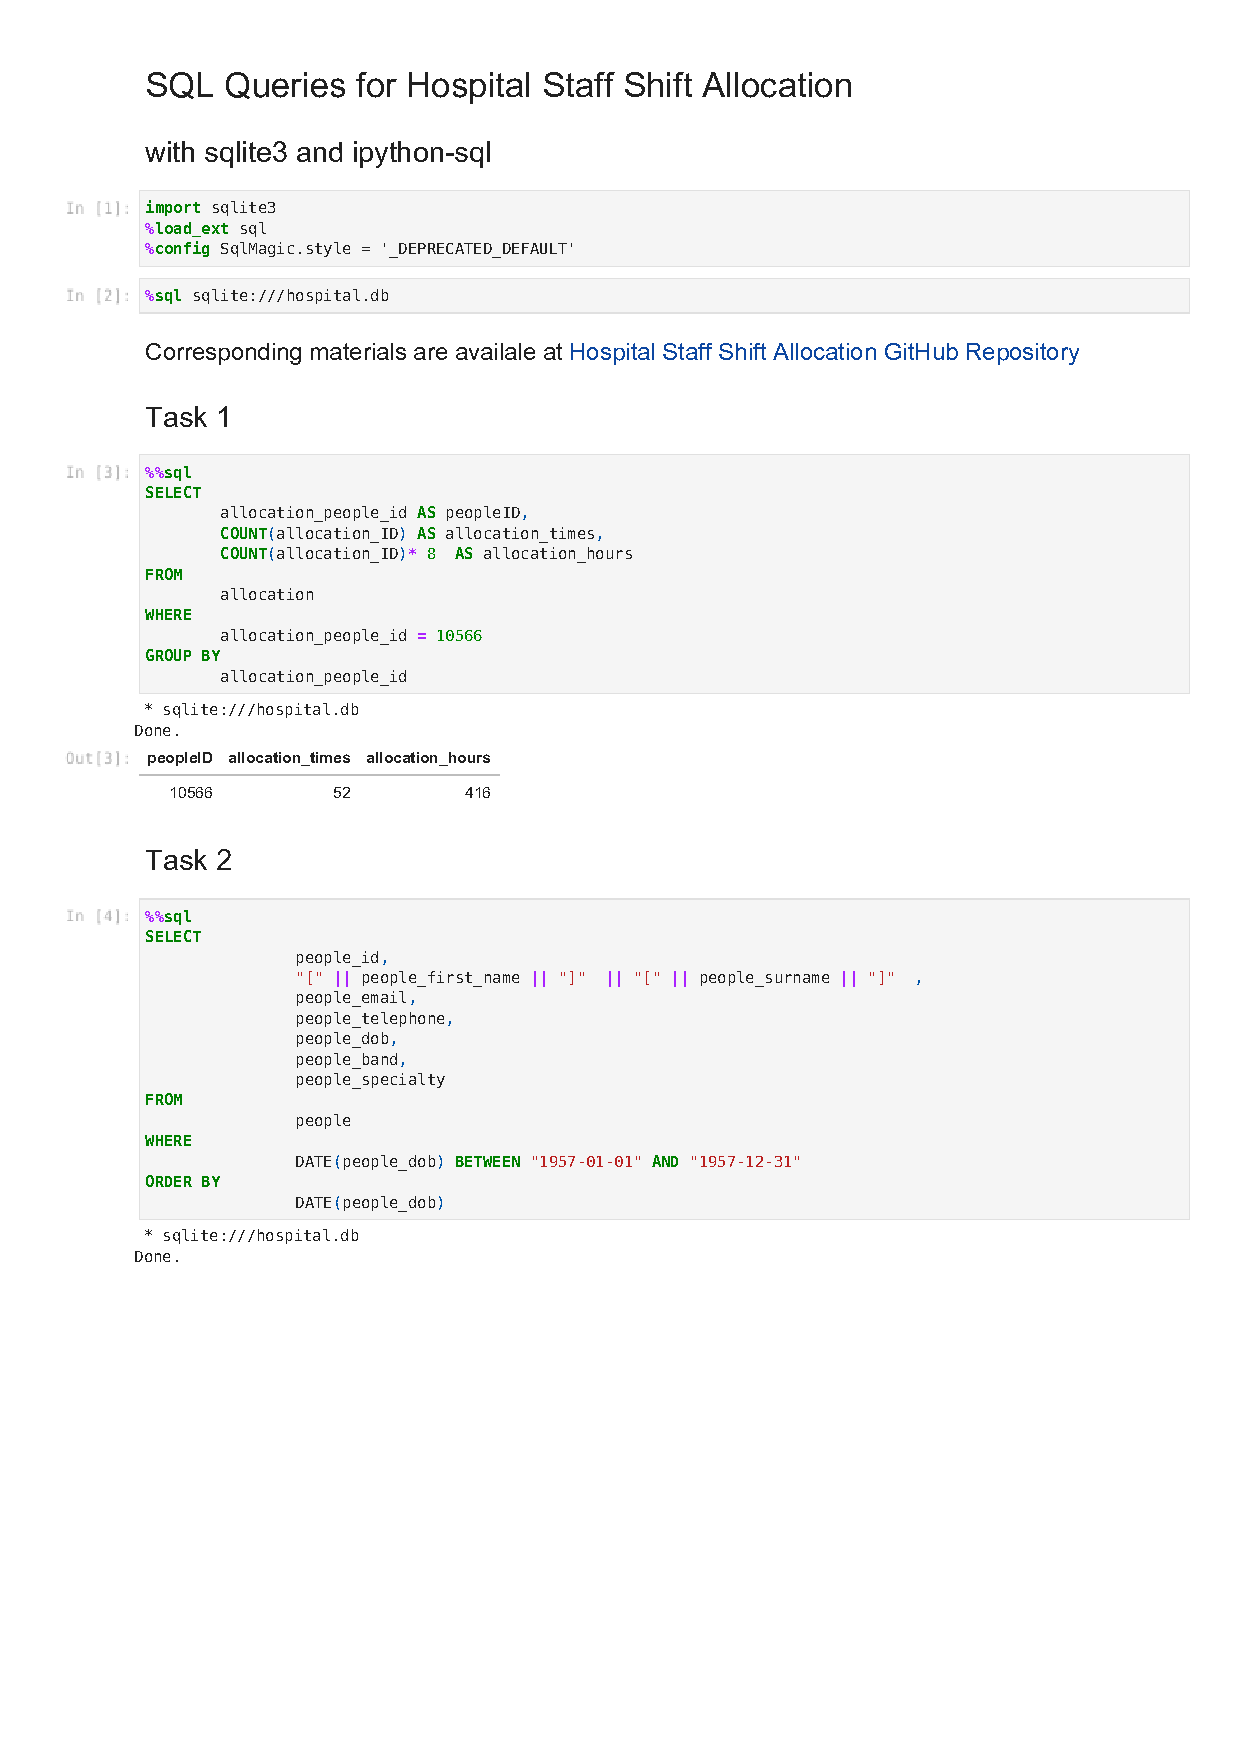
\includepdf[pages=-]{SQL_Queries.pdf}

\end{document}


